\newcommand{\institut}{Institut f\"ur Energie und  Automatisiertungstechnik}
\newcommand{\fachgebiet}{Elektronische Mess- und Diagnosetechnik}
\newcommand{\veranstaltung}{Praktikum Messdatenverarbeitung}
\newcommand{\pdfautor}{\"Ozg\"u Dogan (326 048), Timo Lausen (325 411), Boris Henckell (325 779)}
\newcommand{\autor}{\"Ozg\"u Dogan (326 048)\\ Timo Lausen (325 411)\\ Boris Henckell (325 779)}
\newcommand{\pdftitle}{Praktikum Messdatenverarbeitung  Termin 5}
\newcommand{\prototitle}{Praktikum Messdatenverarbeitung \\ Termin 5}
\newcommand{\aufgabe}{}

\newcommand{\gruppe}{Gruppe: G1 Fr 08-10}
\newcommand{\betreuer}{Betreuer: J\"urgen Funk}

\input{../../packages/tu_header_8}
%\begin{document}

% \lstlistoflistings
\definecolor{darkgray}{rgb}{0.95,0.95,0.95}
\definecolor{darkolivegreen}{HTML}{01a801}
\definecolor{functionsBlue}{HTML}{32b9b9}
\definecolor{variableRed}{rgb}{1,0,0}
\definecolor{stringBrown}{HTML}{bc8e8e} % f geht nicht

\lstset{
        %\lstset{extendedchars=true} % Umlaute an der richtigen stelle und nicht am Anfang ausgeben
        %basicstyle=\footnotesize\ttfamily,
        basicstyle=\small,
        %
        inputencoding=utf8,
        %
        tabsize=4,
        showspaces=false,
        showtabs=false,
        showstringspaces=true, % no special string spaces
        %
        backgroundcolor=\color{darkgray}, % background
        stringstyle=\color{stringBrown}\fseries, % Strings
        keywordstyle=\color{functionsBlue}\bfseries, % keywords Blau
        identifierstyle=\color{variableRed}, % variablen
        commentstyle=\color{darkolivegreen}, %  comments
        %
        breaklines=true,
        %
        numbers=left,
        numberstyle=\tiny,
        stepnumber=1,
        numbersep=7pt,
        %
        frame=single,
        columns=flexible,
        %
        xleftmargin=-2cm,
        xrightmargin=-1.5cm,
        %
        language=Matlab
}


%---------------------------------------------------------------------
%---------------------------------------------------------------------
%---------------------------------------------------------------------


\section{Vorbereitungsaufgaben}
\begin{quote}
    
    \subsection{Vorbereitungsaufgaben zu Termin 5}
    \begin{quote}
    	
    	\subsubsection{FIR Filter entwerfen}
    	\begin{quote}
		    
			Als erstes sollte ein FIR-Filter entworfen werden, welches mit der MATLAB
			Funktion FIRFilterung realisiert wird. Dabei haben wir im Probedurchlauf einen
			Deltaimpuls verwendet, der durch eine Reihe beliebig gewählter
			Filterkoeffizienten läuft. Die entstandene Impulsantwort sieht folgendermaßen
			aus:
			
			\begin{figure}[H]
		            \centering
		                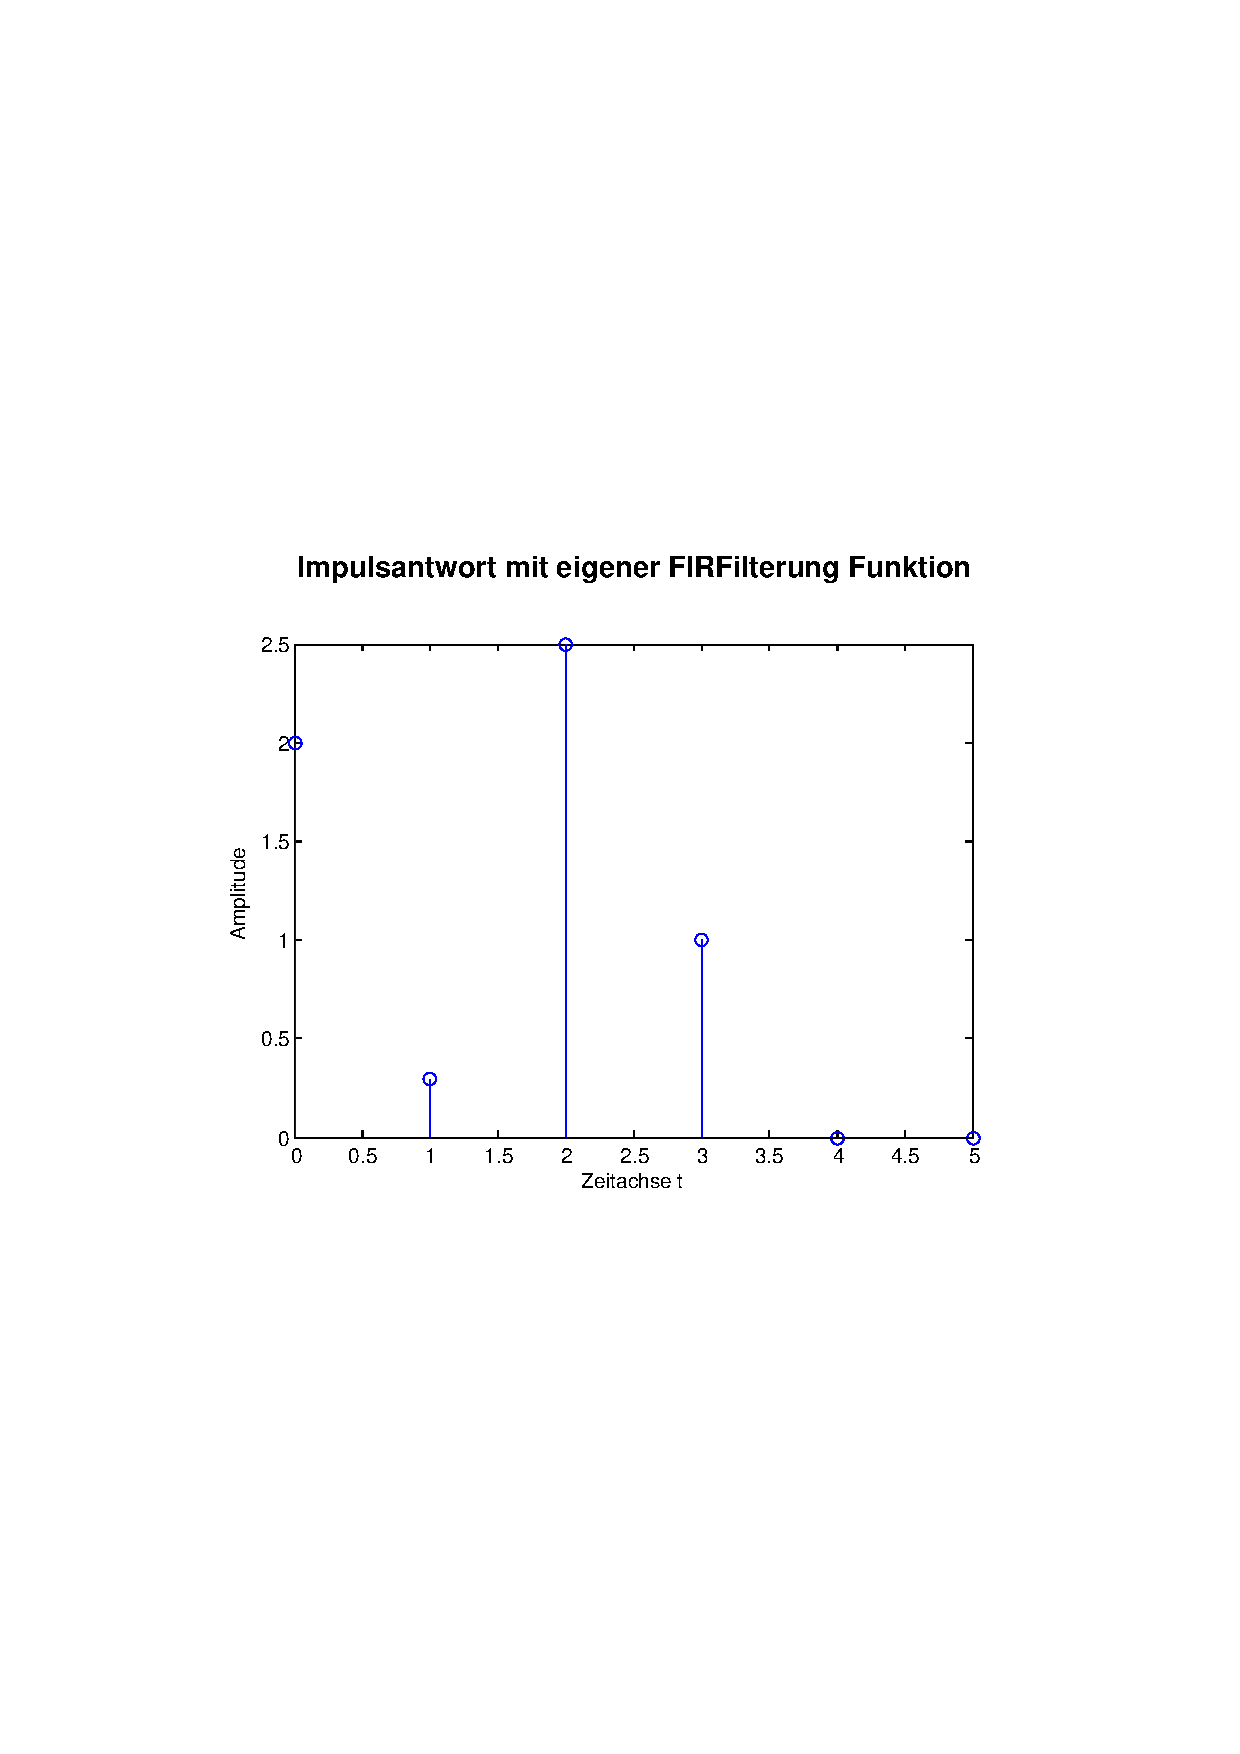
\includegraphics[scale=0.5, trim = 1cm 6cm 1.5cm 8cm,
		                clip]{./Bilder/Impulsantwort_aufgabe1}
		                    \caption{Impulsantwort mit belieben Filterkoeffizienten}
		                    \label{fig:./Bilder/Impulsantwort_aufgabe1}
		            \end{figure}
		            
			Dieses Ergebnis sollte mit dem Vergleich des Ergebnisses der MATLAB
			Buil-in Funktion filter überprüft werden. Das wichtige dabei ist es die
			Rückkopplungskoeffizienten der filter-Methode im ersten Eintrag zu $1$ und den
			Rest zu $0$ zu setzen, damit die Funktion des Filters weiter ohne Rückkopplung
			realisiert werden kann. Mit dem selben Deltaimpuls und den
			bereits verwendeten Filterkoeffizienten erhalten wir den gleichen Plot:
			
			\begin{figure}[H]
		            \centering
		                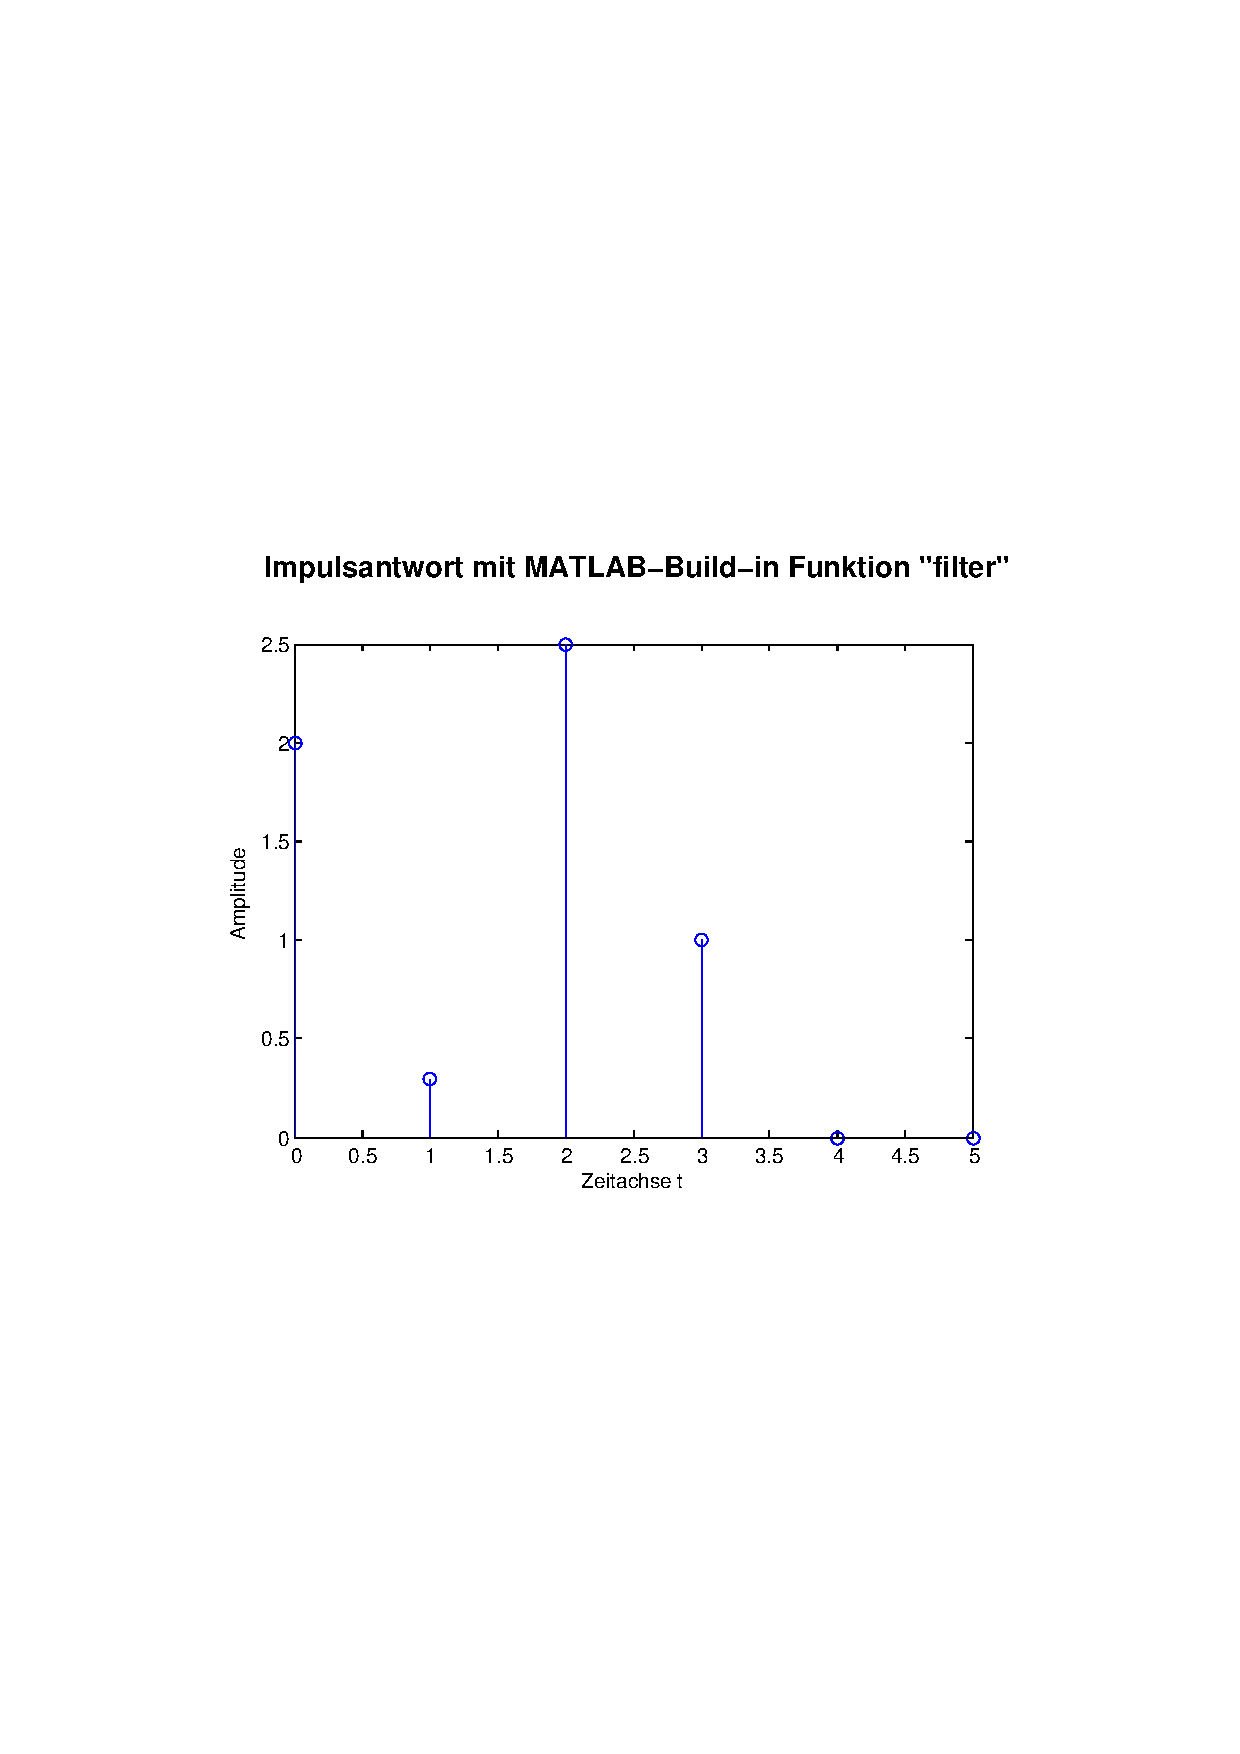
\includegraphics[scale=0.5, trim = 1cm 6cm 1.5cm 8cm,
		                clip]{./Bilder/Impulsantwort_aufgabe11}
		                    \caption{Impulsantwort mit anhand filter-Methode}
		                    \label{fig:./Bilder/Impulsantwort_aufgabe11}
		            \end{figure}
		       
		  \end{quote}   
		  
		  \subsubsection{FIR Filter nach der Fenstermethode entwerfen}
		  \begin{quote}
		            
		    Danach sollte ein FIR-Filter nach der Fenstermethode entworfen werden. Dabei
		    wird der Etwurf Schritt für Schritt selber durchgeführt. Die Vorgabe war es,
		    ein Tiefpass zu bauen, welcher alle Frequenzanteile oberhalb von $1,5 kHz$
		    mit mindestens $60 dB$ dämpft und Frequenzanteile bis zu einer Grenzfrequenz
		    von $1 kHz$ mit maximal $3 dB$ dämpft. Die Abtastfrequenz des TP sollte
		    dabei $15 kHz$ betragen. Untersucht haben wir dabei ein Hanningfenster, ein
		    Blackmanfenster, ein Hammingfenster und ein Rechteckfenster.
		    
		            
		            
		  \end{quote}          
		            
		  \subsubsection{Nachabtastung}
		  \begin{quote}
		            
		    Nun wurde eine Funktion entworfen, mit der sowohl die digitale Filterung als
		    auch das Nachabtasten des Signals realisiert wird. Dabei wird nur jeder
		    fr-ter Wert weiterhin übernommen.  
		 
		  \end{quote}
		  
		  \subsubsection{Verzicht auf analoges Anti-Aliasing-Filter?}
		  \begin{quote}
		  
		  Zuletzt sollte eine Antwort auf die Frage gegeben werden, ob durch den
		  Einsatz eines digitalen Filters ganz auf die Verwendung eines analogen
		  Anti-Aliasing Filters verzichtet werden kann. Die Antwort lautet nein. Durch
		  korrekte Anpassung des digitalen Filters mit ausreichend hoher Ordnung kann zwar 
		  Aliasing beim digitalen Filtern vermieden werden, doch braucht man bei der
		  Digitalisierung des Signals vor der Filterung einen Schutz vor Aliasing,
		  welcher nur durch ein analoges Anti-Aliasing Filter möglich ist.
		  
		  \end{quote}
	
	\end{quote}
	
	
    \subsection{Vorbereitungsaufgaben zu Termin 6}
    \begin{quote}
    	
    	\subsubsection{Beschreibung der Funktion filterFIR}
    	\begin{quote}
    	
    	Die Funktion FilterFIR filtert ein gemessenes Signal. Bei Aufruf wird der n-te Eintrag des gefilterten Signals
    	ausgegeben und der Index incrementiert.\\
    	Die Filterfunktion ist mit einer for-Schleife realisiert. Folgende Schritte werden innerhalb eines Durchlaufs
    	durchgeführt.\\
    	Zu Beginn wird der n-te Messwert aus dem Buffer geholt. Dieser ursprüngliche Messwert hat 10 Bit und keine
    	Nachkommastellen. Um 6 weitere Nachkommastellen zu erhalten wird dieser um 6 Stellen nach links geshiftet. Im
        nächsten Schritt wird der Wert mit dem entsprechenden Filterkoeffizenten multilpliziert. Alle Filterkoeffizenten
        sind 16 Bit groß haben 15 Nachkommastellen. Bei der multiplikation von zwei 16 Bit Zahlen ergibt sich eine 32
        Bit Zahl. Das Ergebniss besitzt nach der multiplikation 21 Nachkommastellen. Für die weitere Rechnung werden die
        letzten 16 Nachkommastellen vernachlässigt. Die Ergebnisse aller multiplikationen werden zum endergebniss
        aufaddiert. Daraus resultiert das gefilterte Signals an der Stelle n.\\
        Nach vollendung wird der n-te Messwert aus dem Speicher gelöscht. Dadurch wird beim nächsten Aufruf der n+1 -te
        Messwert gefiltert.\\
        Abschließend werden die noch verbleibenden 5 Nachkommastellen abgeschnitten und das gerundete Ergebniss
        zurückgegeben.
        
		\end{quote}
		
		\subsubsection{}
		\begin{quote}
		
		\ldots
		
		\end{quote}
		
		\subsubsection{}
		\begin{quote}
		
		\ldots
		
		\end{quote}
				
\end{quote}%Ende Vorbereitunsaufgaben zu Termin 5

\section{Durchführungen}
\begin{quote}
		
		\subsection{Durchführung zu Termin 5}
		\begin{quote}
			
			Im praktischen Teil des 5. Labortermins, sollte untersucht werden, wie die
			Abtastrate eines Signals durch Nachabtastung (Dezimation) verringert werden
			konnte.
			
			\subsubsection{Aufnahme eines Rechtecksignals}
			\begin{quote}
			
			Zuerst sollte ein Rechtecksignal aufgenommen werde, welche eine Frequenz von
			$110 Hz$ besaß. Die Abtastrate betrug $15 kHz$ und es wurde ein analoges
			Anti-Aliasing Filter verwendet. Danach wurde das Amplitudenspektrum des
			Signals bestimmt und bis zu einer Frequenz von $1 kHz$ geplottet. 
			
			\end{quote}%Ende Aufnahme eines Rechtecksignals
			
			\subsubsection{Dezimation des Rechtecksignals}
			\begin{quote}
			
			Nun wurde eine Dezimation durchgeführt, in dem das Signal mittels eines MATLAB
			Skriptes nochmal mit einer Frequenz von $3 kHz$ abgetastet wurde. Somit
			erhielten wir jeden fünften Wert aus dem aufgenommenen Signal und konnten
			die die restlichen Werte verwerfen, wodurch die Datenmenge deutlich
			verkleinert wurde. Nach der Abtastung wurde erneut das Amplitudenspektrum
			ermittelt, bis $1 kHz$ dargestellt und mit dem Amplitudenspektrum aus der
			vorherigen Aufgabe verglichen.
			
			\end{quote}%Ende Dezimation des Rechtecksignals
			
			\subsubsection{digitale Filterung des Rechtecksignals}
			\begin{quote}
			
			Als nächstes wurde das Rechtecksignal mit dem in der Vorbereitungsaufgabe
			entworfenem digitalen Filter (zunächst ohne Dezimation) gefiltert und manuell
			mit der Abtastrate von $3 kHz$ dezimiert. Danach wurde wieder das
			Amplitudenspektrum bis $1 kHZ$ gebildet und mit den Ergebnissen aus den
			vorherigen Aufgaben verglichen.
			
			\end{quote}%Ende digitale Filterung des Rechtecksignals
			
			\subsubsection{Testen der Funktion DecimFilt}
			\begin{quote}
			
			Zuletzt haben wir die ebenfalls in der Vorbereitungsaufgabe entworfene
			Funktion DecimFilt auf das aufgenommene Rechtecksignal angewendet, wodurch das
			Signal automatisch erst gefiltert und dann mit der Abtastrate von $3 kHz$
			dezimiert wurde. Wieder wurde das erzielte Amplitudenspektrum mit den anderen
			Amplitudenspektren verglichen.
			
			\end{quote}
		\end{quote}
		
		\subsection{Durchführung zu Termin 6}
		\begin{quote}
		
		\end{quote}
		
\end{quote}%Ende Durchführungen


%--------------------------------------------------------------------
%--------------------------------------------------------------------
%--------------------------------------------------------------------
%--------------------------------------------------------------------
\section{Quellcodes}
\begin{quote}

	\subsection{Codes aus Termin 5}
	\begin{quote}
	    \subsubsection{FIRfilterung.m}
	    \begin{quote}
	        \lstinputlisting[
	            caption={FIRfilterung},
	            label=lst:Matlab]
	            {./Matlab/FIRfilterung.m}
	    \end{quote}
	    
	    \subsubsection{Fenstermethode.m}
	    \begin{quote}
	        \lstinputlisting[
	            caption={Fenstermethode},
	            label=lst:Matlab]
	            {./Matlab/Fenstermethode.m}
	    \end{quote}
	    
	    \subsubsection{DecimFilt.m}
	    \begin{quote}
	        \lstinputlisting[
	            caption={DecimFilt},
	            label=lst:Matlab]
	            {./Matlab/DecimFilt.m}
	    \end{quote}
	    
	\end{quote}
\end{quote}

%--------------------------------------------------------------------
%--------------------------------------------------------------------


%\begin{thebibliography}{999}
%\bibitem {Schaltungwandlerbox} Prof. Dr.-Ing. Gühmann, Clemens; Dipl.-Ing. Funk, Jürgen: MDVLaborGeraete_web, S.4

%Name, Vorname.; evtl. Name2, Vorname2.: Titel des Dokumentes
%oder Buches, Zeitschrift/Verlag/URL (Auflage, Erscheinungsort, -jahr), ggf. Seitenzahlen
%\bibitem {PasevalscheTheorem} \url{https://de.wikipedia.org/wiki/Parsevalsches_Theorem}, Zugriff
%23.05.2012
%\end{thebibliography}


\end{document}


